\section{The Calorimeters}
\label{sec:calo}

\subsection{Electromagnetic Calorimeter}
\label{subsec:ecal}

% WHAT IT IS
\textit{\textbf{What is it?}}
Particles that pass through the silicon tracker~\ref{sec:tracker} encounter the electromagnetic calorimeter (ECAL).
Those particles which interact electromagnetically but not strongly, mostly photons and electrons, are typically absorbed by the ECAL.
The particle's energy is then transferred to the ECAL in the form of an electromagnetic (EM) shower.
The size and shape of the EM shower provide information about the particle's energy and trajectory.
Since the Higgs boson can decay into two photons, it was essential that the ECAL was able to detect this decay mode.

% STRUCTURE
\textit{\textbf{Structure:}}
The ECAL is a hermetic, cylindrical, homogeneous sub-detector that consists of a barrel (EB), two endcaps (EE), and a preshower detector in front of each endcap (Figure~\ref{fig:ecal_xs}, Left).
The EB covers $\abseta < 1.479$ while the EE covers $1.479 < \abseta < 3.0$.
The entire subdetector is composed of transparent lead tungstate (PbWO$_4$) crystals that point axially towards the center of CMS (the interaction point).
The transparent crystals, one of which is shown in Fig.~\ref{fig:ecal_crystals} (Left), have a high density (8.28 g/\cm$^3$) which provides the ECAL with radiation resistance and a short radiation length ($X_0 = 0.89 \cm$).
Because so many crystals are used (61,200 crystals in the EB and 7,324 in the EE), the ECAL has excellent energy resolution and fine granularity.
Each endcap is composed of two ``Dee''s, one of which is shown in Figure~\ref{fig:ecal_xs} (Right).
A single Dee carries 3,662 crystals.
Crystals in the barrel are tapered, having front face dimensions $2.2 \times 2.2 \cm^2$, back face dimensions $2.6 \times 2.6 \cm^2$, and are 23.0 \cm long (25.8 $X_0$).
Crystals in the endcaps are also tapered, with front face dimensions $2.862 \times 2.862 \cm^2$, back face dimensions $3.0 \times 3.0 \cm^2$, and are 22.0 \cm long (24.7 $X_0$).
This gives a single crystal from the barrel a volume of approximately 132.5 \cm$^3$ (mL), about the volume of a small cup of coffee, yet it weighs 1.5 Kg.
(REF:PDG).
REF:PDG
Particle Data Group collaboration, S. Eidelman \etal., \textit{Review of particle physics},
\textit{Phys. Lett. \textbf{B 592 (2004) 1}}

% ECAL diagram
\begin{figure*}[!htb]
    \centering
    \captionsetup{justification=justified}
    % 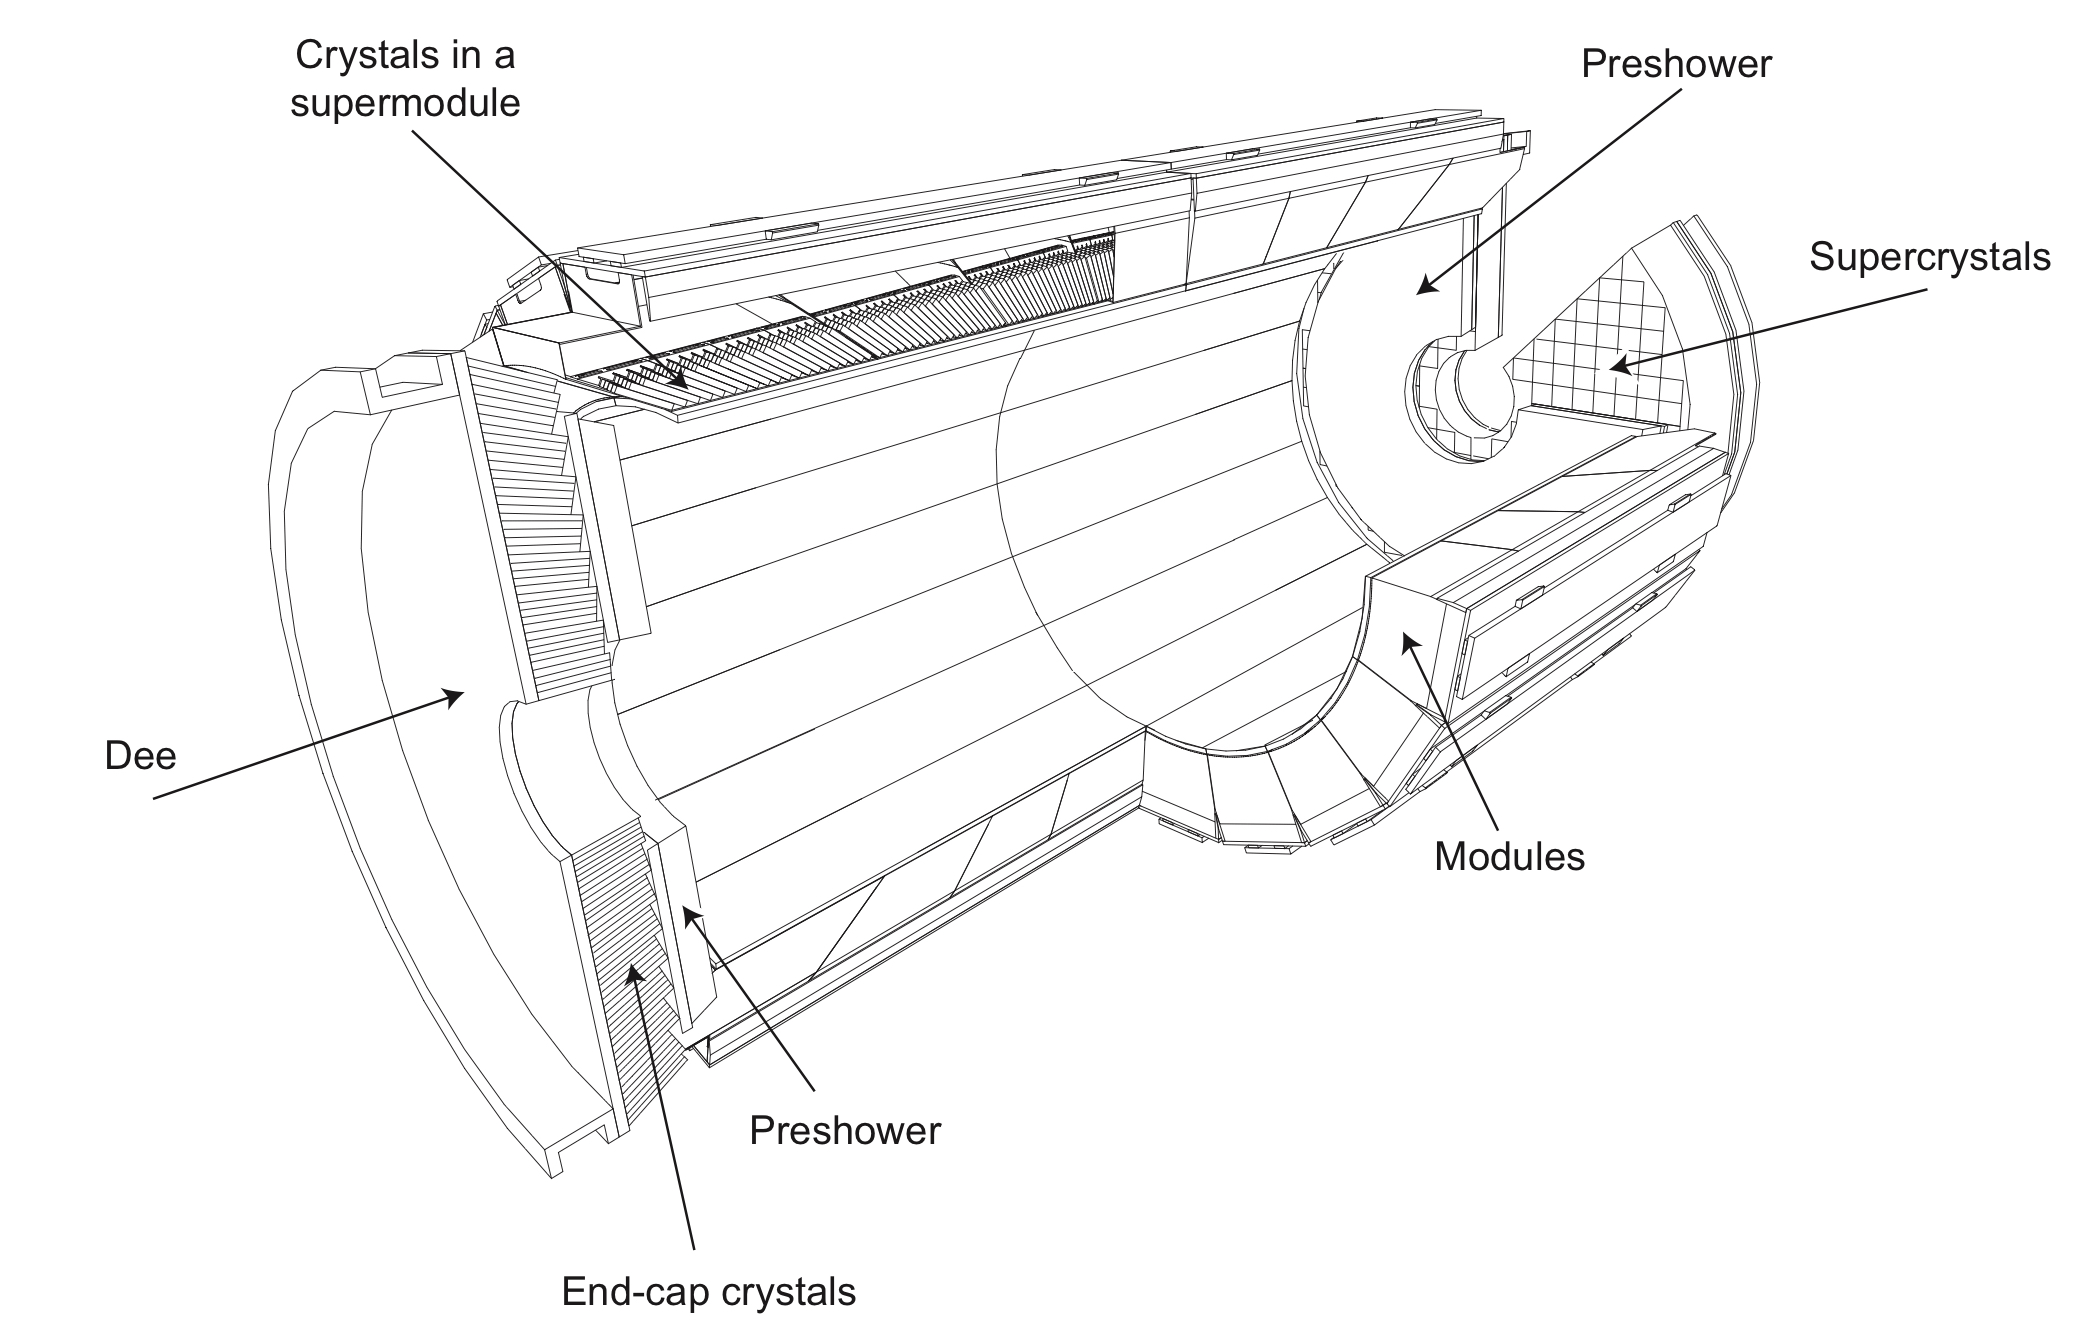
\includegraphics[width=0.95\textwidth]{figures/cms/ecal/xs_whiteblack.jpeg}
    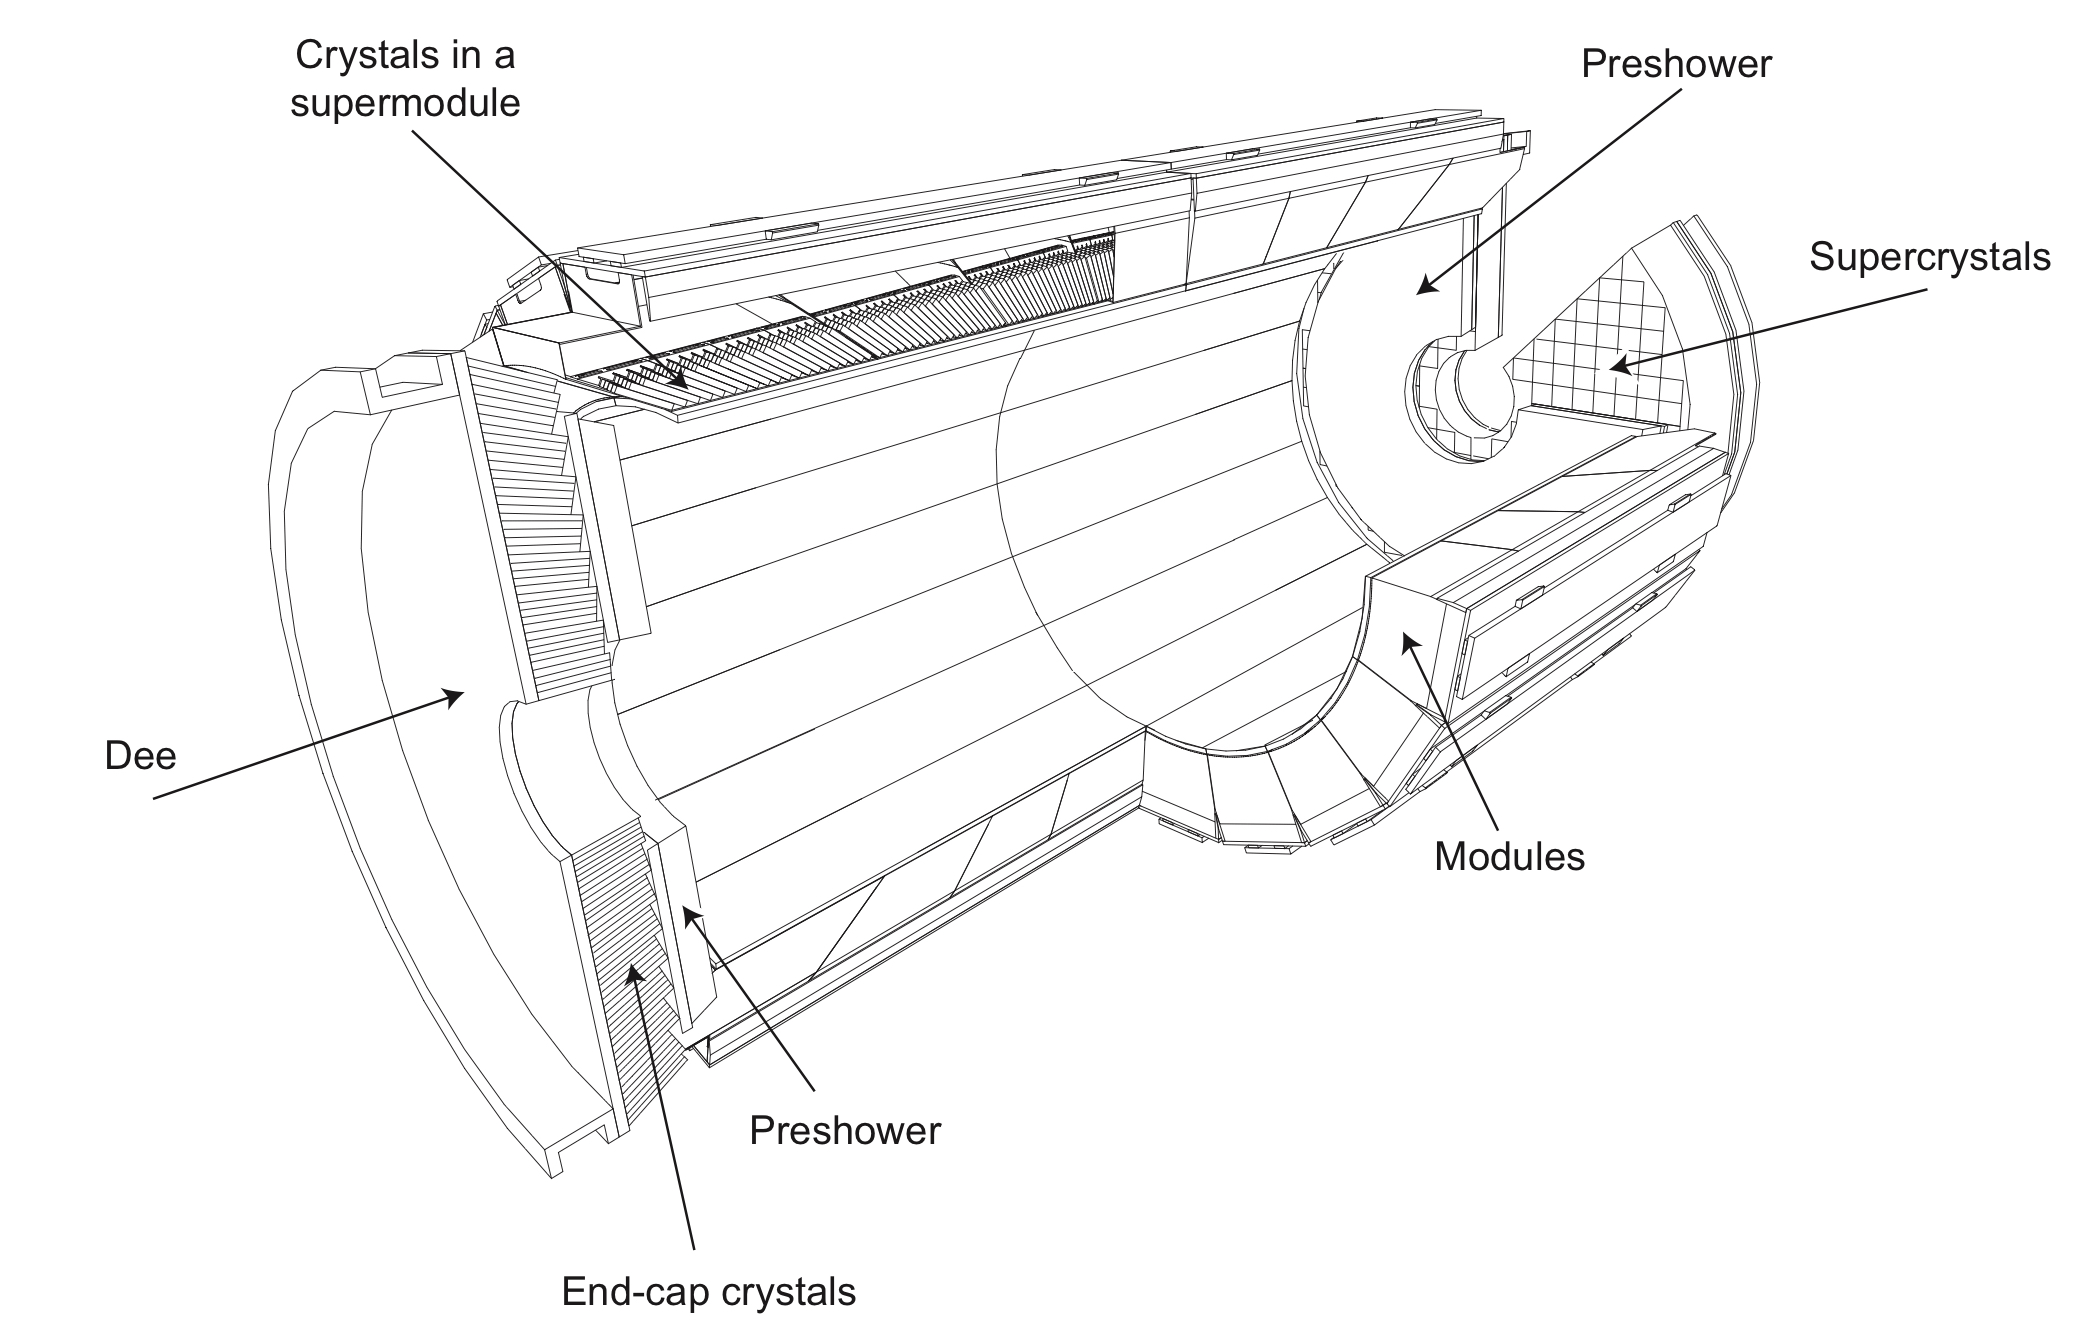
\includegraphics[width=0.49\textwidth,height=10cm,keepaspectratio]{figures/cms/ecal/xs_whiteblack.jpeg}
    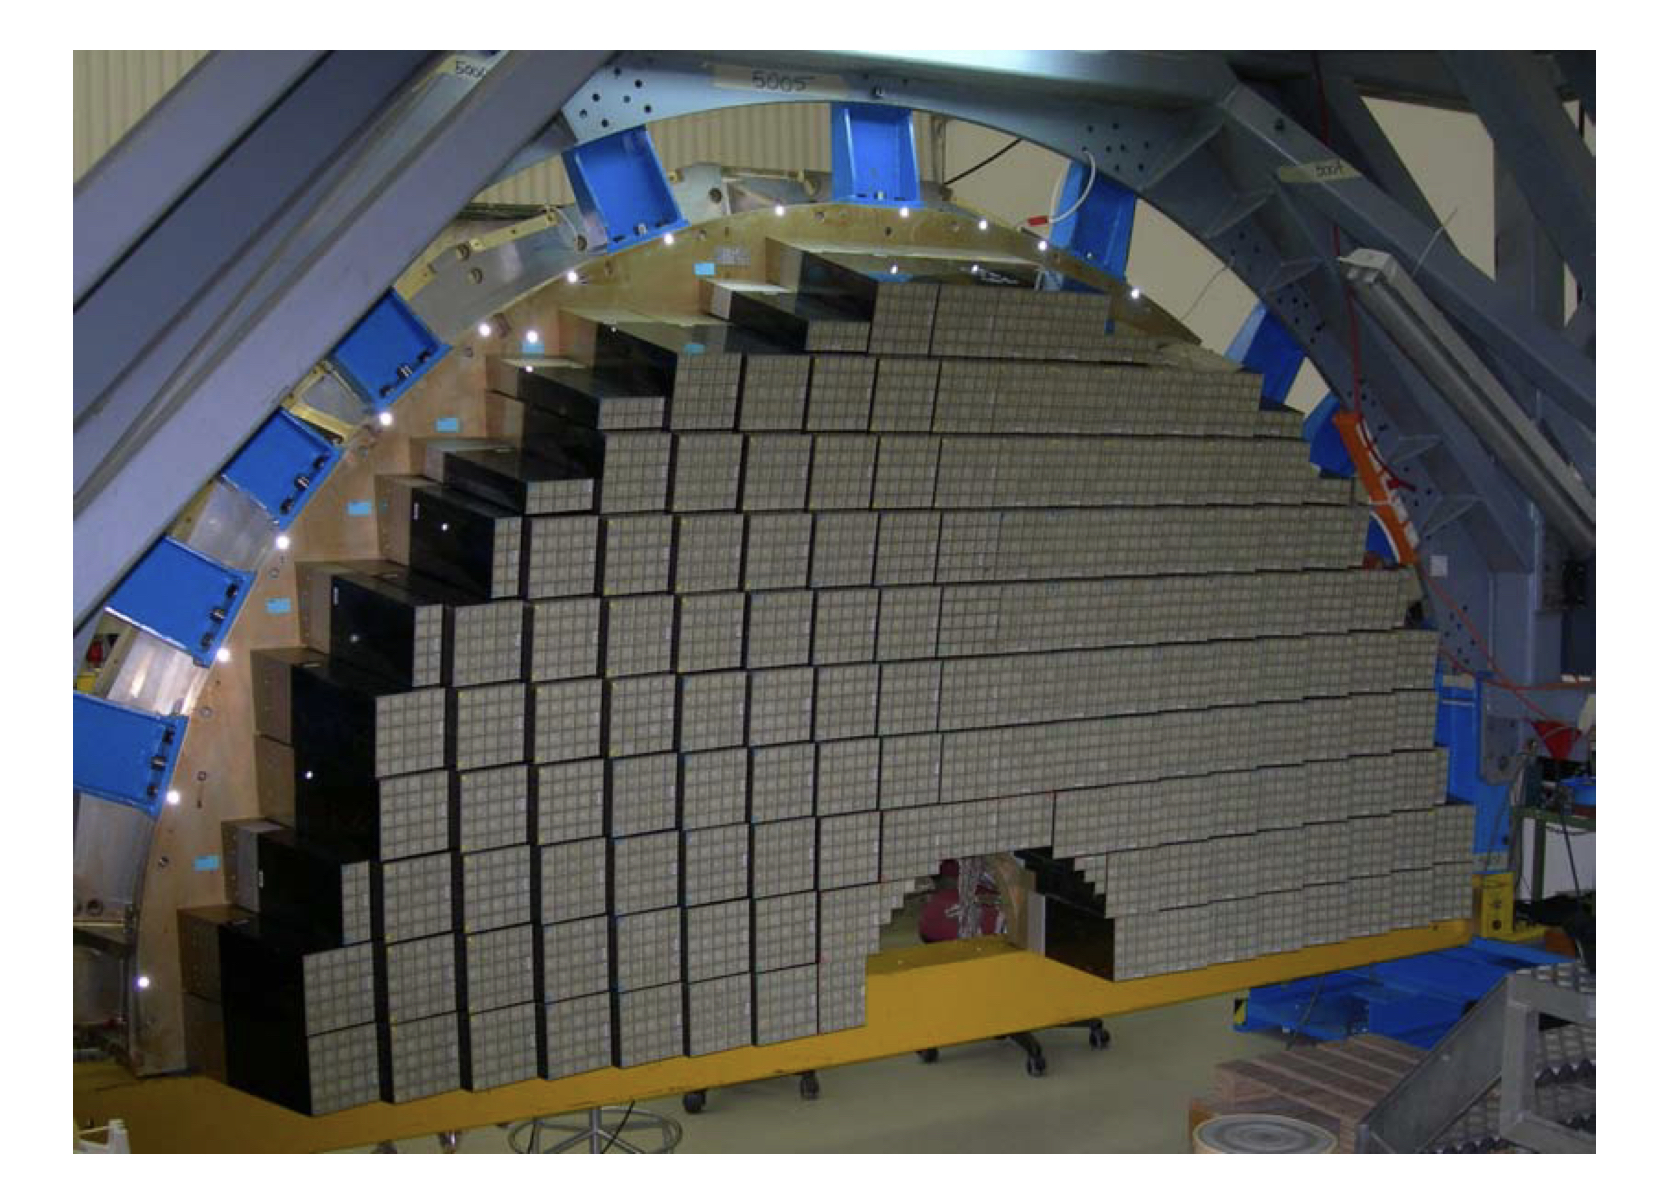
\includegraphics[width=0.49\textwidth,height=10cm,keepaspectratio]{figures/cms/ecal/dee.jpeg}
    \caption{
        (Left) Cross sectional view of the electromagnetic calorimeter of CMS.
        (Right) One of the Dees which comprise the EE.
        Each square of $ 5 \times 5$ crystals constitutes a ``supercrystal''.
        Figure taken from Ref.REFERENCE JINST%  ~\cite{jinst:cms_exp}.
        }
    \label{fig:ecal_xs}
\end{figure*}

%%%%%%%%%%%%%%%%%%%%
% ECAL Crystals
\begin{figure}[pbth]
    \centering
    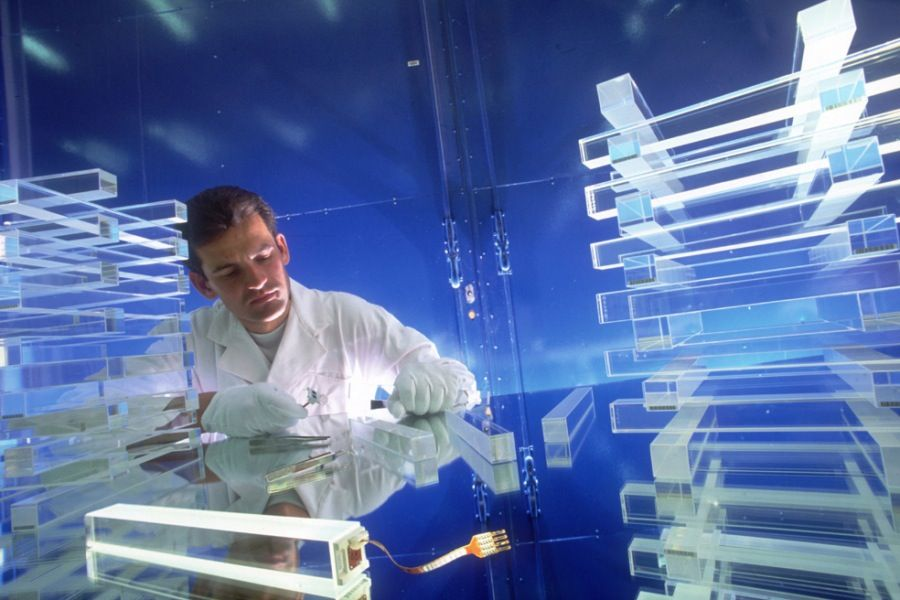
\includegraphics[width=0.49\textwidth,height=10cm,keepaspectratio]{figures/cms/ecal/ECAL_crystals_fancy_lab.jpg}
    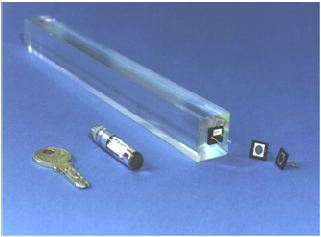
\includegraphics[width=0.49\textwidth,height=10cm,keepaspectratio]{figures/cms/ecal/ECAL_crystal_sizecomparison.jpg}
    \caption{
        (Left) ECAL crystals made from PbWO$_4$ are grown in a lab.
        (Right) Although made mostly of metal, ECAL crystals are transparent and have a photomultiplier detector attached at the end.} 
    \label{fig:ecal_crystals}
\end{figure}
%%%%%%%%%%%%%%%%%%%%

% PHYSICS
\textit{\textbf{Physics:}}
When electrons or photons pass through the ECAL, they create an EM shower.
Electrons radiate more photons as they accelerate around PbWO$_4$ nuclei, in a process called \emph{bremsstrahlung}.
Meanwhile, near the presence of a nucleus, high-energy photons pair produce into \ee.
% In turn, these newly-produced electrons can radiate more photons 
This cycle of electron and photon production disperses the initial particle energy into a spray of lower- and lower-energy particles; an EM shower (REFERENCE EM SHOWER FIG).

SHOW PICTURE OF EM SHOWER.

The ECAL crystals then scintillate (emits photons) in proportion to the amount of energy deposited by the interacting particle. 
The scintillator photons are detected by avalanche photodiodes on the back of each barrel crystal or by vacuum phototriodes in the endcap crystals (Fig.~\ref{fig:ecal_crystals}, Right).
Conveniently after 1 bunch crossing (25 ns), Approximately 80\% of the scintillated light is emitted.

An energy deposit in the ECAL could come from either an electron or a photon.
In order to tell the difference, information from the silicon tracker is used.
Charged particles, like electrons, will leave hits in the tracker and follow a curved path, whereas photons are electrically neutral and thus will not show any signs within the silicon tracker.
So long as the tracker and ECAL communicate effectively with each other, then they help distinguish between electrons and photons.
Charged hadrons interact only minimially with the ECAL, instead continuing on to the Hadron Calorimeter.
Neutral hadrons can be detected by the ECAL preshower near the ECAL endcaps which helps distinguish a single photon from $\pi^{0}$ mesons as they decay into two photons with a narrow opening angle, making it look as if the two photons are a single photon.
The preshower detector allows CMS to distinguish between low-energy diphoton pairs and single high-energy photons.

NEED SMOOTH TRANSITION INTO HCAL. What about those hadrons? They got through the ECAL... To detect hadrons effectively, we need a Hadron Calorimeter.
% That's what we see here with the blue dashed line (the photon) and the red line (the positron).

\subsection{Hadron Calorimeter}

% WHAT IT IS
\textit{\textbf{What is it?}}
The particles that survive the ECAL, typically only muons and hadrons, then enter the hadron calorimeter (HCAL).
Its primary purpose is to absorb the hadronic matter emerging from the interaction point.
The absorbed jet energies cause the HCAL to scintillate photons which are then converted into electrical signals.
These signals are used to deduce the original jet energies and any missing transverse energy (\MET) from the event.
% emit proportionally-energetic scintillated 

% STRUCTURE
\textit{\textbf{Structure:}}
Dissimilar to the ECAL (subsec.~\ref{subsec:ecal}) in material composition but similar in shape, the HCAL is a brass cylindrical scintillator.
So although it has a barrel (HB) and two endcaps (HE), the HCAL also has an outer calorimeter (HO), and a forward calorimeter (HF) close to the beam pipe.
With a thickness of over $1~\meter$, the HB is sandwiched between the barrels of the ECAL and the solenoid (subsec.~\ref{sec:solenoid}) at radial values $r = 1.77~\meter$ and $r = 2.95~\meter$, respectively.
Because the HB and HE are located within the solenoid's strong magnetic field of 3.8 T, they both were both constructed out of a non-magnetic absorber called \emph{C26000 cartridge brass}.
This absorber has a density of 8.53 $\g/\cm^{3}$ and an interaction length $(\lambda_I)$ of 16.42~\cm, which yields approximately 7.2(?) $(\lambda_I)$ within the thickness of the HB.
The HB spans the pseudorapidity range $\abseta < 1.3$, the HE spans $1.3 < \abseta < 3$, and the HF spans $3 < \abseta < 5.2$, as shown in Figure~\ref{fig:hcal_quadrant}.
Since the volume available to the HCAL is so limited, and in order to stop any particles that might traverse the entire HCAL and solenoid, the HO (the so-called ``tail catcher'') is situated outside the barrel of the solenoid.
The HF is located 

How many layers?
What is a tray?
delta eta delta phi = (0.087, 0.087)

%%%%%%%%%%%%%%%%%%%%
% HCAL Quadrant
\begin{figure}[pbth]
    \centering
    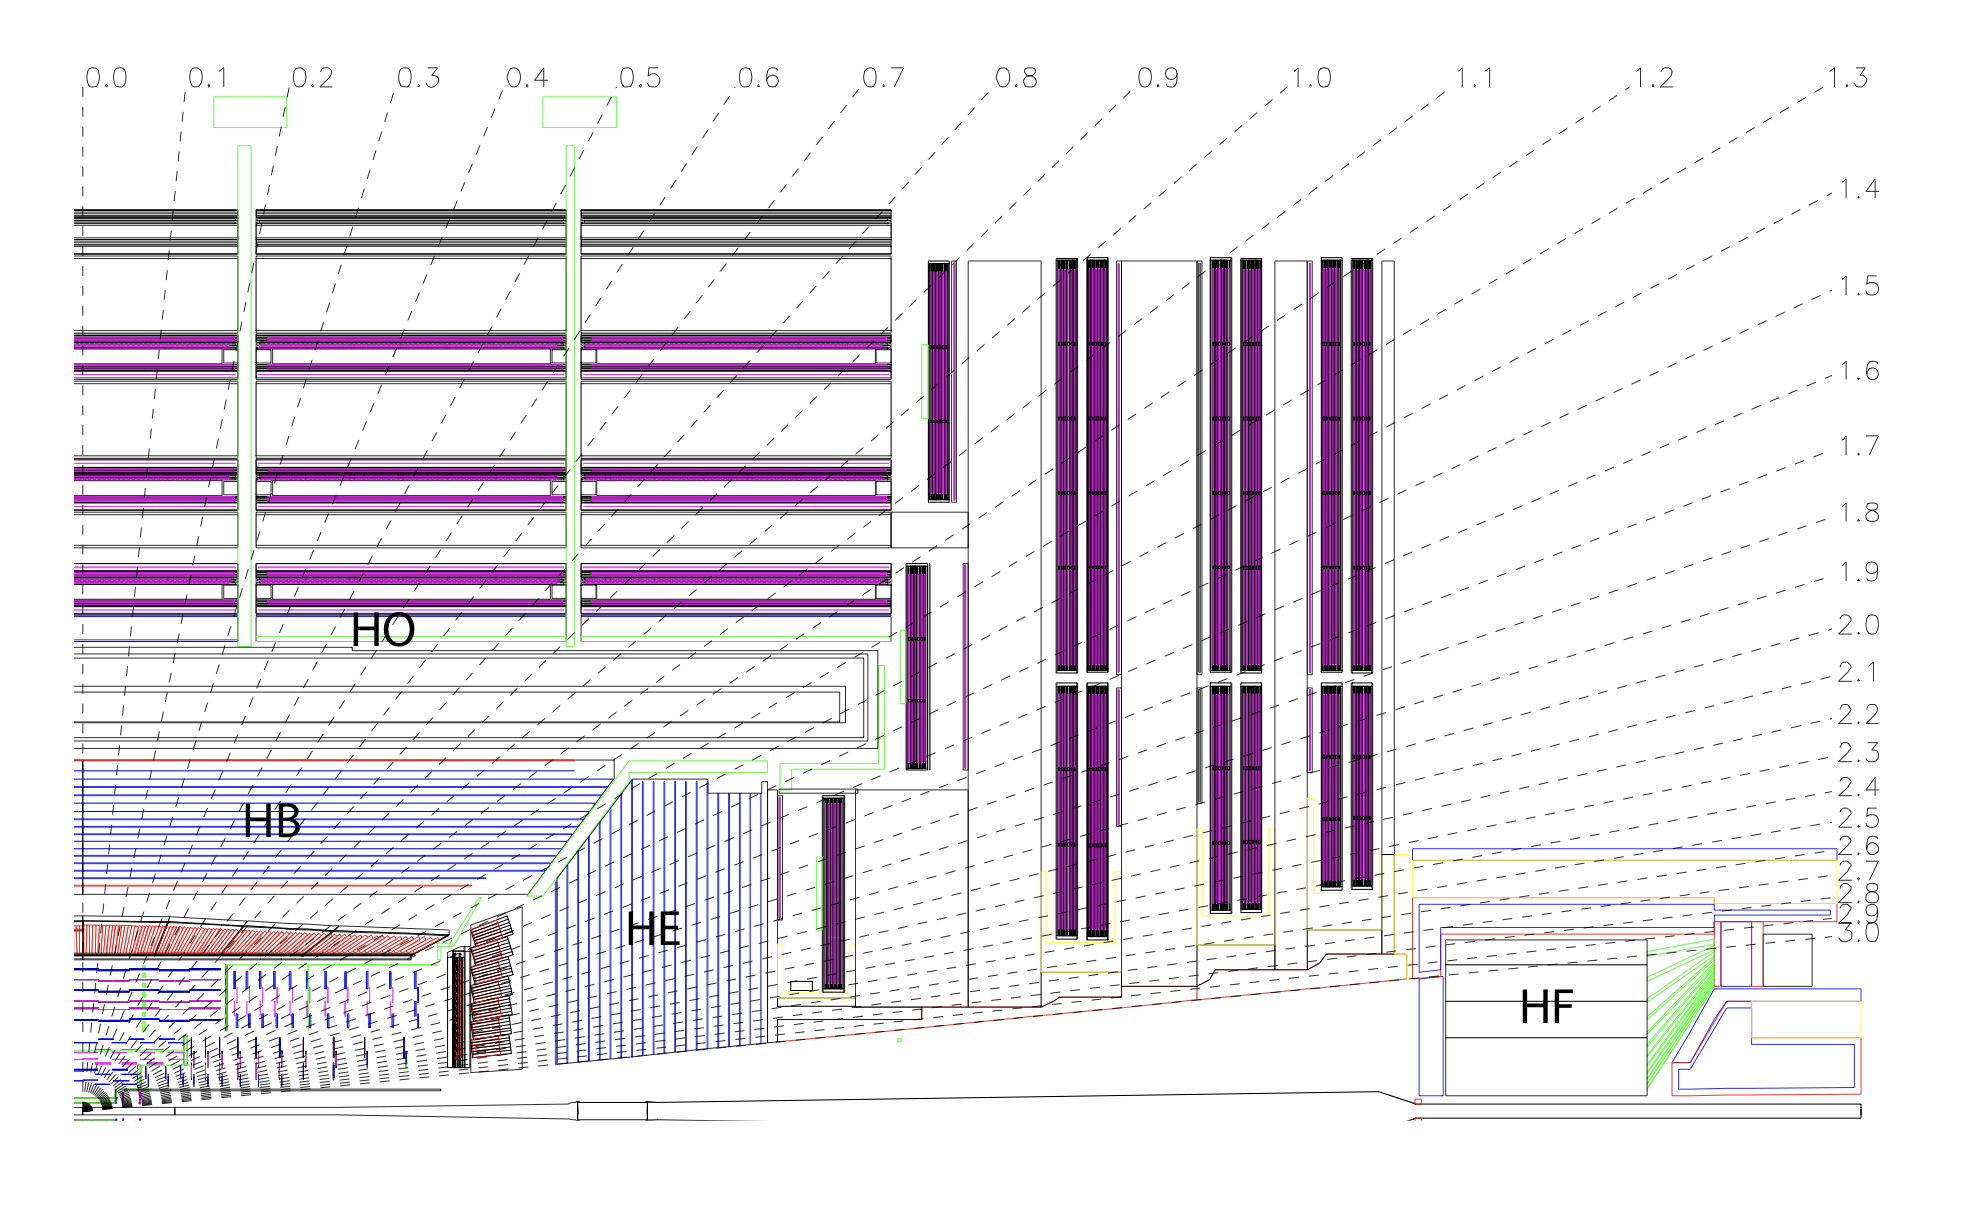
\includegraphics[width=0.95\textwidth]{figures/cms/hcal/hcal_quadrants_longitudinalview.jpg}
    \caption{
        A cross-sectional quadrant of CMS showing the locations of the HCAL components:
        the barrel (HB), outer (HO), endcap (HE), and forward (HF) detectors.
        }
    \label{fig:hcal_quadrant}
\end{figure}
%%%%%%%%%%%%%%%%%%%%

% PHYSICS
\textit{\textbf{Physics:}}
Hadrons interact via the strong force with the Similar to the ECAL, the HCAL will scintillate in proportion to the amount of energy of the captured particle. 
The incoming hadrons will \emph{hadronize} (\ie, produce a hadronic shower), generating jets of quarks and gluons which are bound in various ways forming protons, neutrons, pions, kaons, \etc
Interestingly, the HCAL is made using over a million old, brass shell casings from the Russian Navy back from World War II.
% kinds of particles which have not decayed on their own or were not caught by the ECAL, ,  or when it catches hadronic material: stuff made of quarks, like . 

About 34\% of the particles produced from LHC \pp collisions enter the HE region, so the HE was built to handle high rates (MHz).

The entire HCAL utilizes approximately 70,000 tiles.
